\documentclass[convert, tikz]{standalone}
%\usepackage{xcolor}
\begin{document}
%\pagecolor[RGB]{255,255,254}
  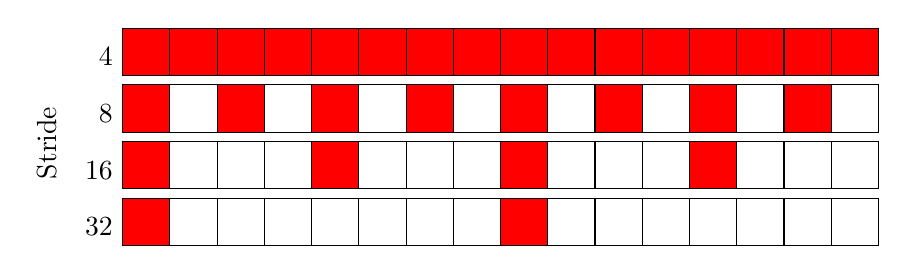
\begin{tikzpicture}[scale=0.6]
    \begin{scope}
      \node[above left] (0,1) {4};
      \draw(0,0) grid(16,1);
      \foreach \i in {0,...,15}{
          \draw[fill=red] (\i,0) rectangle (\i+1,1);
       }
    \end{scope}
    \begin{scope}[yshift=-1.2cm]
      \node[above left] (0,1) {8};
      \draw(0,0) grid(16,1);
      \foreach \i in {0,2,...,14}{
          \draw[fill=red] (\i,0) rectangle (\i+1,1);
       }
    \end{scope}
    \begin{scope}[yshift=-2.4cm]
      \draw(0,0) grid(16,1);
      \node[rotate=90,above right] at (-12mm,0) {Stride};
      \node[above left] (0,1) {16};
      \foreach \i in {0,4,...,12}{
          \draw[fill=red] (\i,0) rectangle (\i+1,1);
       }
    \end{scope}
    \begin{scope}[yshift=-3.6cm]
      \node[above left] (0,1) {32};
      \draw(0,0) grid(16,1);
      \foreach \i in {0,8}{
          \draw[fill=red] (\i,0) rectangle (\i+1,1);
       }
    \end{scope}
  \end{tikzpicture}
\end{document}
